\begin{frame}[fragile]{Tutorial: n-site operators with MPO}

\begin{columns}

\begin{column}{5cm}

\begin{onlyenv}<1->
\begin{lstlisting}[language=JuliaLocal, style=julia, mathescape, basicstyle=\scriptsize\ttfamily]
function ising(n; h)
  H = OpSum()
  for j in 1:(n - 1)
    H -= "Z", j, "Z", j + 1
  end
  for j in 1:n
    H += h, "X", j
  end
  return H
end

h = 0.5 # field
H = MPO(ising(n; h), i)
maxlinkdim(H) == 3
\end{lstlisting}
\end{onlyenv}

\begin{onlyenv}<3->
\begin{lstlisting}[language=JuliaLocal, style=julia, mathescape, basicstyle=\scriptsize\ttfamily]
Zp = MPS(i, "Zp")
inner(Zp', H, Zp) == -(n-1)
 \end{lstlisting}
\end{onlyenv}

\end{column}

\begin{column}{5.5cm}

\begin{onlyenv}<1-1>
$n$ sites \\
$H = -\sum_j^{n-1} Z_j Z_{j+1} + h \sum_j^n X_j$ \\
~\\
~\\
~\\
~\\
~\\
~\\
~\\
~\\
\end{onlyenv}

\begin{onlyenv}<2->
\vspace*{0.0cm}
\begin{center}
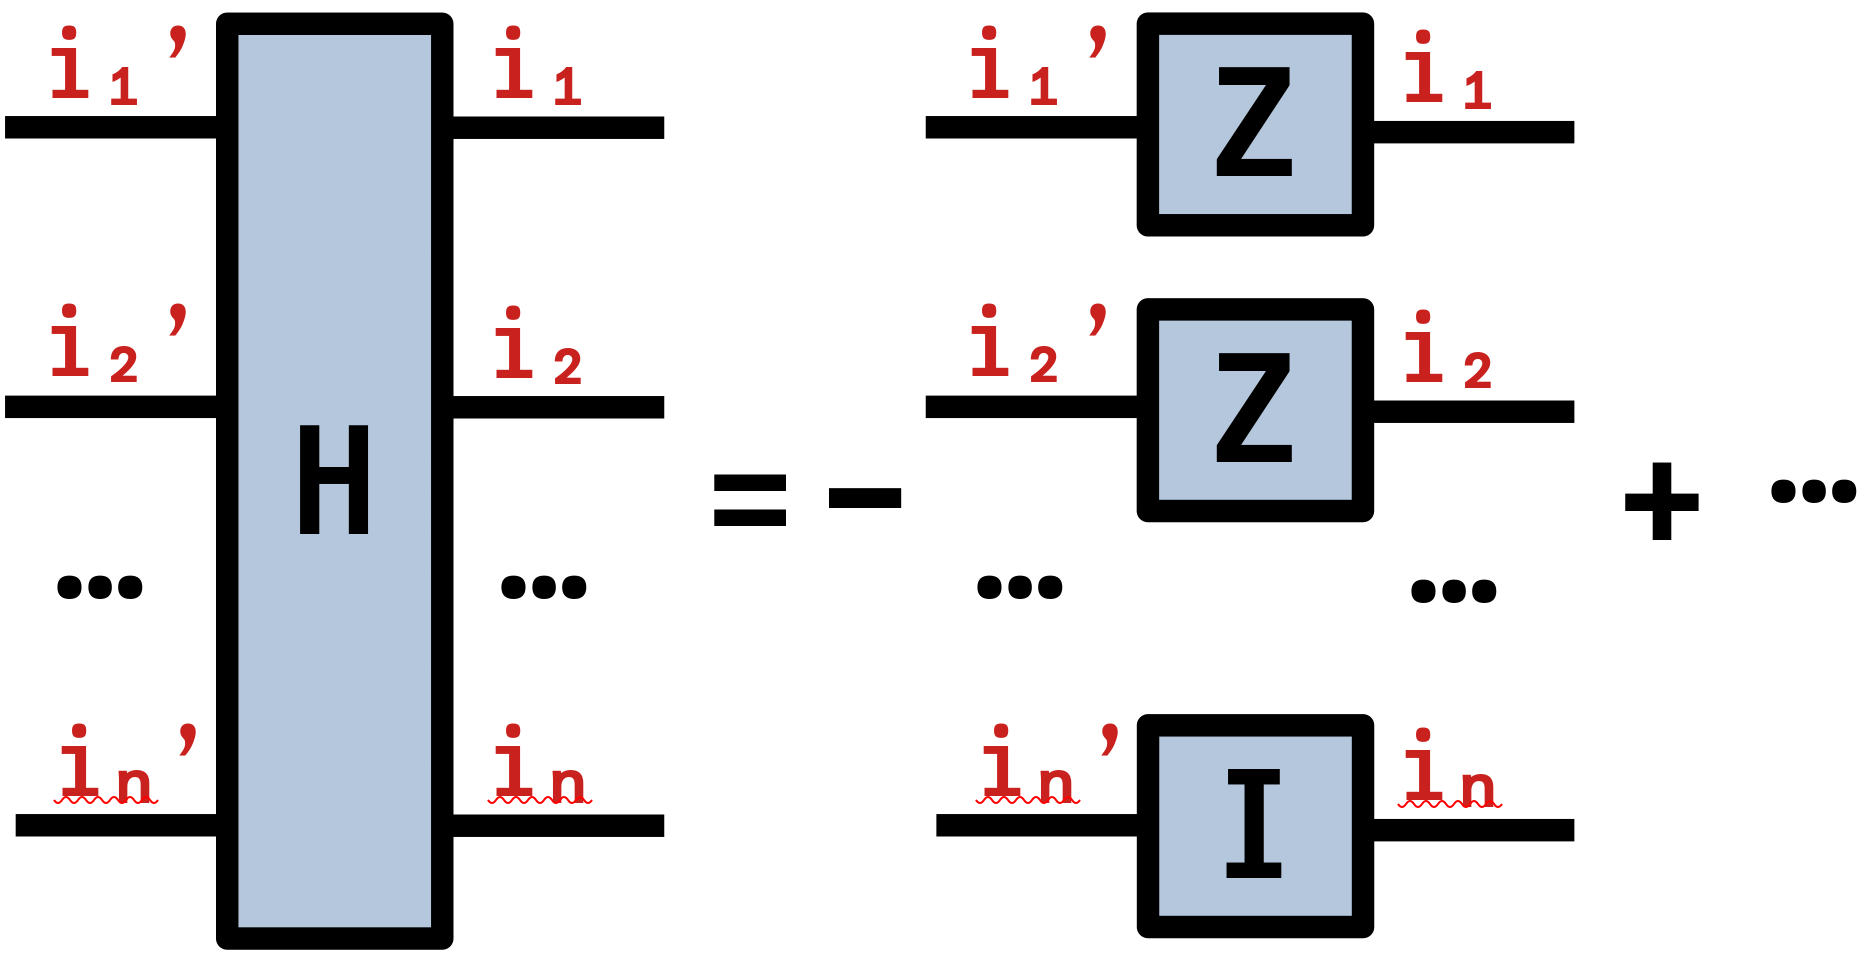
\includegraphics[width=0.64\textwidth]{
  slides/assets/isingn.png
}
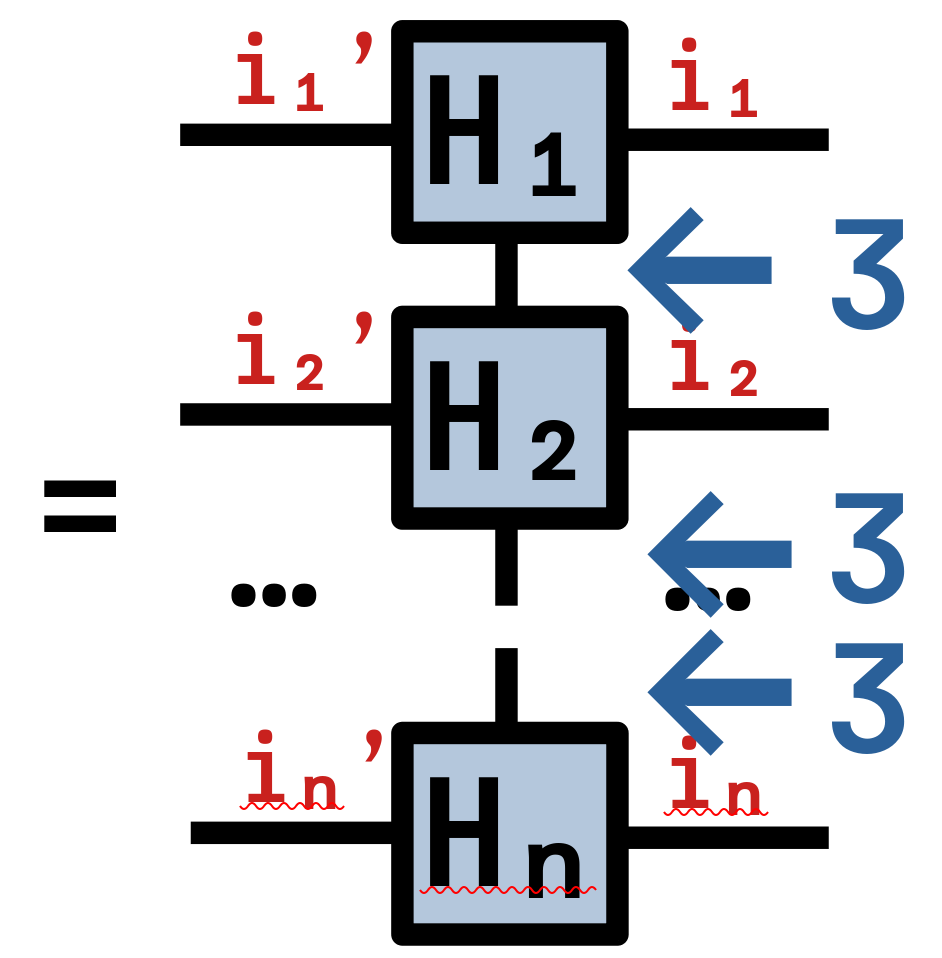
\includegraphics[width=0.33\textwidth]{
  slides/assets/isingn_mpo.png
}
\end{center}
\vspace*{0.0cm}
\end{onlyenv}

%% \begin{onlyenv}<3-3>
%% ~\\
%% ~\\
%% = 3 (local Hamiltonian) \\
%% ~\\
%% $\langle$Z+Z+…Z+|H|Z+Z+…Z+$\rangle$ \\
%%   $\approx$ -(n - 1) = -29
%% \end{onlyenv}

\begin{onlyenv}<3->
\vspace*{0.0cm}
~\\
~\\
\begin{center}
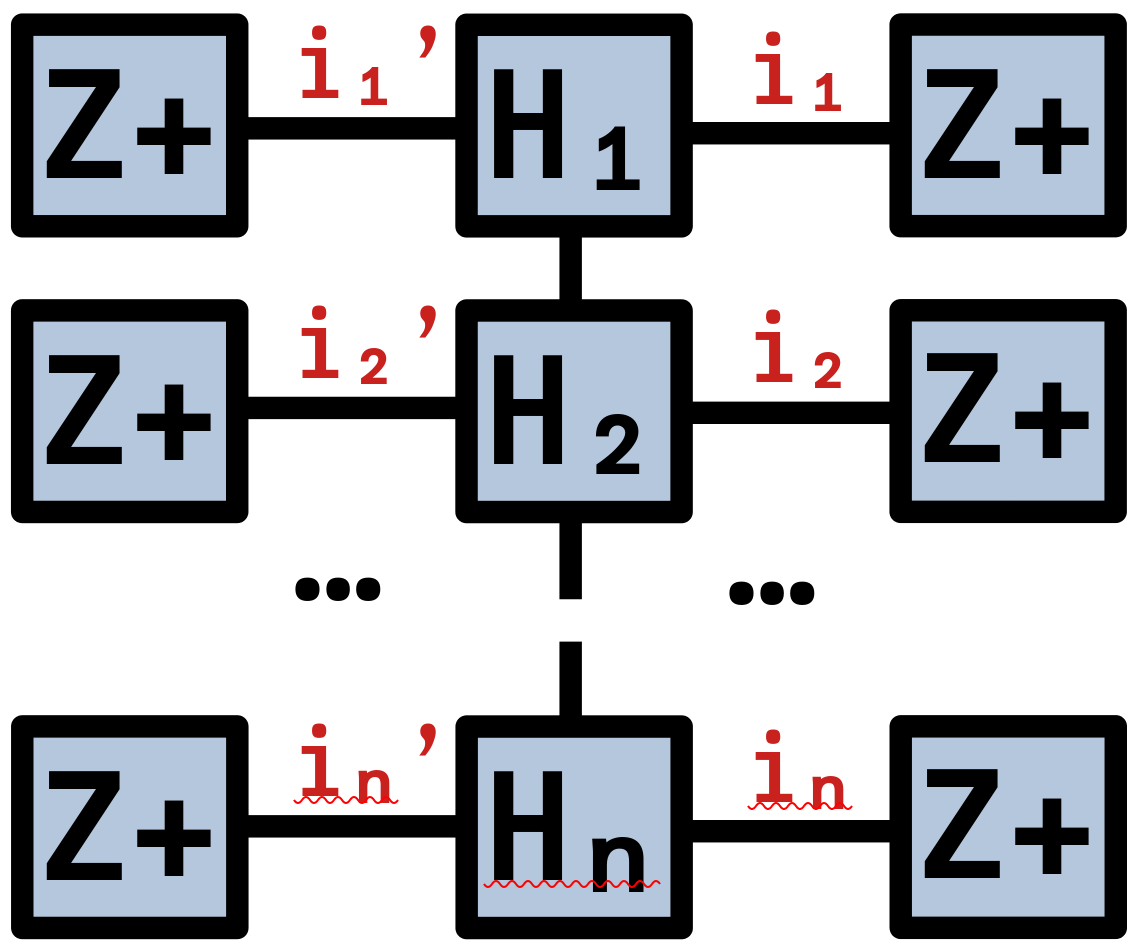
\includegraphics[width=0.48\textwidth]{
  slides/assets/Zpn_H_Zpn.png
}
\end{center}
\vspace*{0.0cm}
\end{onlyenv}
\end{column}

\end{columns}

\end{frame}
